% This file was created with tikzplotlib v0.10.1.
% make bar plot appear once in legend
\pgfplotsset{compat=1.11,
    /pgfplots/ybar legend/.style={
    /pgfplots/legend image code/.code={%
       \draw[##1,/tikz/.cd,yshift=-0.25em]
        (0cm,0cm) rectangle (3pt,0.8em);},
   },
}

\begin{figure}
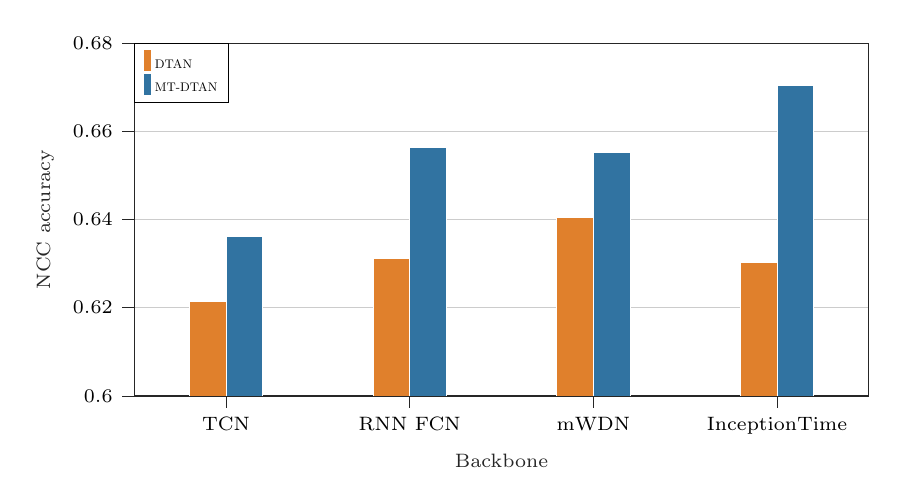
\begin{tikzpicture}

\definecolor{brown1926061}{RGB}{192,60,61}
\definecolor{darkslategray38}{RGB}{38,38,38}
\definecolor{lightgray204}{RGB}{204,204,204}
\definecolor{mediumpurple147113178}{RGB}{147,113,178}
\definecolor{peru22412844}{RGB}{224,128,44}
\definecolor{seagreen5814558}{RGB}{58,145,58}
\definecolor{steelblue49115161}{RGB}{49,115,161}

\begin{axis}[
axis line style={darkslategray38},
tick align=outside,
tick pos=left,
x grid style={lightgray204},
xlabel=\textcolor{darkslategray38}{Backbone},
xlabel style={font=\scriptsize}, % Smaller font for x-label
xmin=-0.5, xmax=3.5,
xtick style={color=darkslategray38},
xtick={0,1,2,3},
xticklabel style={rotate=0.0, font=\scriptsize}, % Smaller font for x-ticks
xticklabels={TCN,RNN FCN,mWDN,InceptionTime},
%legend pos=north west,
legend style={at={(0,1)}, anchor=north west, nodes={scale=0.5, transform shape}, font=\small}, % Smaller font for legend
legend cell align=left,
smooth,
y grid style={lightgray204},
ylabel=\textcolor{darkslategray38}{NCC accuracy},
ylabel style={font=\scriptsize}, % Smaller font for y-label
ymajorgrids,
ymin=0.6, ymax=0.68,
ytick style={color=darkslategray38},
yticklabel style={font=\scriptsize}, % Smaller font for y-ticks
width=0.9\textwidth, height=0.5\textwidth,
]
\draw[draw=white,fill=peru22412844,line width=0.32pt] (axis cs:0,0) rectangle (axis cs:-0.2,0.621518408744956);
\draw[draw=white,fill=peru22412844,line width=0.32pt] (axis cs:1,0) rectangle (axis cs:0.8,0.631102543388569);
\draw[draw=white,fill=peru22412844,line width=0.32pt] (axis cs:2,0) rectangle (axis cs:1.8,0.640454320102535);
\draw[draw=white,fill=peru22412844,line width=0.32pt] (axis cs:3,0) rectangle (axis cs:2.8,0.630160900322637);
\addlegendimage{ybar,ybar legend,draw=white,fill=peru22412844,line width=0.32pt}
\addlegendentry{DTAN}

\draw[draw=white,fill=steelblue49115161,line width=0.32pt] (axis cs:1,0) rectangle (axis cs:1.2,0.656342056075144);
\draw[draw=white,fill=steelblue49115161,line width=0.32pt] (axis cs:2,0) rectangle (axis cs:2.2,0.655250724125139);
\draw[draw=white,fill=steelblue49115161,line width=0.32pt] (axis cs:3,0) rectangle (axis cs:3.2,0.670476629324275);
\draw[draw=white,fill=steelblue49115161,line width=0.32pt] (axis cs:2.77555756156289e-17,0) rectangle (axis cs:0.2,0.636244756503774);
\addlegendimage{ybar,ybar legend,draw=white,fill=steelblue49115161,line width=0.32pt}
\addlegendentry{MT-DTAN}

\end{axis}
% \usetikzlibrary{calc}
% \draw ({$(current bounding box.south west)!0.5!(current bounding box.south east)$}|-{$(current bounding box.south west)!1.1!(current bounding box.north west)$}) node[
%   scale=0.2,
%   anchor=north,
%   text=darkslategray38,
%   rotate=0.0
% ]{Mean NCC Accuray};
\end{tikzpicture}
\caption{DTAN vs. MT-DTAN comparison across different backbones on 113 datasets of the UCR archive~\cite{Dau:2019:ucr} (2019 version) 
evaluated by the Nearest Centroid Classification (NCC) accuracy.}
\label{fig:barplot}
\end{figure}